\documentclass[
    10pt,
    aspectratio=169,
    xcolor={dvipsnames},
    spanish,
    % handout,
    % notes=only,
    % notes,
    ]{beamer}

% BEAMER SETTINGS
\setbeamerfont{section in toc}{size=\normalsize, shape=\bfseries}
\mode<presentation>{
    \usetheme{Antibes}
    \setbeamercovered{transparent}
    \usecolortheme{rose}
    \setbeamertemplate{navigation symbols}{}
    }

% PACKAGES
% \usepackage[spanish]{babel}  % uncomment for Spanish support
\usepackage{tikz,pgfplots}
\pgfplotsset{compat=1.13}
\usetikzlibrary{calc}
\usepackage{subcaption}
\usepackage{graphicx}
\graphicspath{{figures}}
\usepackage{booktabs}
\usepackage{upgreek}
\usepackage{commath}
\usepackage{amsmath,amsthm,amssymb,mathtools,mathrsfs}
\usepackage{cancel}
\usepackage{fontawesome5}
\usepackage{enumerate}
\usepackage{tensor}
\usepackage[font=footnotesize]{caption}
\usepackage{wasysym}

\usepackage[skins,theorems]{tcolorbox}
\tcbset{
    highlight math style={
        enhanced,
        coltext=black,
        colframe=black,
        colback=lightgray,
        arc=0pt,
        boxrule=.5pt
        }
}

% REFERENCES AND OTHERS
\usepackage{aas_macros}
\usepackage{natbib}
\bibpunct{(}{)}{;}{a}{}{,}

\usepackage{siunitx}
\sisetup{
    range-phrase=\text{--},
    range-units=single,
    separate-uncertainty=true,
    print-unity-mantissa=false
    }
\DeclareSIUnit{\gauss}{G}
\DeclareSIUnit{\jansky}{Jy}
\renewcommand{\figurename}{Fig.}

\usepackage{hyperref}
\hypersetup{
    % bookmarks=true,
    unicode=true,
    pdftoolbar=true,
    pdfmenubar=true,
    pdffitwindow=false,
    pdfstartview={FitH},
    pdftitle={ISI-Free Linear Combination Pulses with Better Performanc},
    pdfauthor={Erik Saez A.},
    pdfcreator={Erik Saez A.},
    pdfnewwindow=true,
    colorlinks=true,
    linkcolor=RoyalBlue,
    citecolor=RoyalBlue,
    urlcolor=RoyalBlue
    }

\title[Auxiliar \#1 - Análisis de señales]{\bfseries Auxiliar \#1 - Análisis de señales}
\subtitle{}
\author[Erik Saez A.]{Erik Saez A.}
\institute[UChile]{Department of Electrical Engineering \\ Universidad de Chile}

\date{\today}

\begin{document}

\begin{frame}
  \titlepage
  \centering
  \faIcon{envelope} \href{mailto:erik.saez@ug.uchile.cl}{erik.saez@ug.uchile.cl} \hspace{.2cm}
\end{frame}

\begin{frame}
  \frametitle{Contenidos}
  \centering
  \begin{columns}
    \begin{column}{0.4\textwidth}
      \tableofcontents
    \end{column}
    \begin{column}{0.5\textwidth}
      \begin{figure}
        \centering
        
\includegraphics[width=\textwidth]{fcfm_die}
        \caption{Facultad de Ciencias Físicas y Matemáticas , Universidad de Chile.}
      \end{figure}
    \end{column}
  \end{columns}  
\end{frame}
%%%%%%%%%%%%%%%%%%%%%%%%%%%%%%%%%%%%%%%%%%

\section{Motivación}
\begin{frame}{Motivación}
  \begin{itemize}
    \item ¿Por qué vale la pena tomar este ramo?
    \item ¿Qué me puede aportar si no pienso dedicarme al área de Telecomunicaciones?
    \item ¿Es realmente importante ir a clases? 
    \item ¿Qué cosas interesantes voy a aprender aquí?
    \item ¿Cómo se relaciona con sistemas de comunicación modernos?
    \item \dots
  \end{itemize}
\end{frame}
%%%%%%%%%%%%%%%%%%%%%%%%%%  
\section{Aspectos Generales del curso}


%%%%%%%%%%%%%%%%%%%%%%%%%%%
\begin{frame}{Continuidad del ramo}
  \begin{itemize}
    \item Análisis de señales $\rightarrow$ Principios de Comunicaciones / Fundamentos de control de Sistemas
    \item ¡Atrasa! pero no es crítico (¡Si para los del área de Telecomunicaciones, cuidado!)
    \item Base fundamental para: modulación, codificación, filtrado digital, etc.
  \end{itemize}
  \begin{figure}
    \centering
    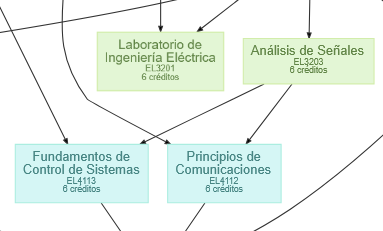
\includegraphics[width=0.5\textwidth]{Figura_1.png}
    \caption{Continuidad del ramo}
  \end{figure}
\end{frame}
%%%%%%%%%%%%%%%%%%%%%%%%%
\begin{frame}{Evaluaciones del ramo}
\begin{columns}
  \begin{column}{0.5\textwidth}
    \begin{block}{Tipos de Evaluación}
      \begin{table}[h]
        \centering
        \footnotesize
        \begin{tabular}{|l|l|}
        \hline
        \textbf{Tipo} & \textbf{Descripción} \\
        \hline
        Tareas (5) & Actividades semanales \\
        \hline
        Proyectos 1 y 2 & Proyectos de desarrollo \\
        \hline
        Controles (3) y Examen & Evaluaciones  \\
        \hline
        \end{tabular}
      \end{table}
    \end{block}
  \end{column}
  
  \begin{column}{0.43\textwidth}
    \begin{alertblock}{Recomendaciones}
      \footnotesize
      \begin{itemize}
        \item Controles: Harta matemática y teoría
        \item Los ejercicios no dejarlos para último momento
        \item Proyectos son largos, por lo que prepararlos con anticipación
      \end{itemize}
    \end{alertblock}
  \end{column}
\end{columns}
\end{frame}
%%%%%%%%%%%%%%%%%%%%%%%%

%%%%%%%%%%%%%%%%%%%%%%%%%
\begin{frame}{}
\begin{center}
\Huge ¿Alguna duda?
\end{center}
\end{frame}
%========================
\section{Unidad 1: Introducción}
\begin{frame}{Señales: Definición Formal}
\begin{columns}[T,onlytextwidth]
  % ===== Columna texto
  \begin{column}{0.5\textwidth}
    \begin{block}{Concepto}
    \begin{itemize}
      \item Una \textbf{señal} es una función de tiempo.
      \item \textbf{Tiempo continuo}: \(x(t): \mathbb{R} \rightarrow \mathbb{R}^{\alpha}\).
      \item \textbf{Tiempo discreto}: \(x[n]: \mathbb{Z} \rightarrow \mathbb{R}^{\alpha}\).
    \end{itemize}
    \end{block}

    \begin{block}{Definición}
      \footnotesize
    Un \textbf{sistema} es un operador que transforma una señal de entrada en una señal de salida.
    \[
    \begin{aligned}
    T_c&:\ \mathcal{S}(\mathbb{R},\mathbb{R}^{\alpha}) \to \mathcal{S}(\mathbb{R},\mathbb{R}^{q}),
    &\qquad y(t)&=(T_c\{x\})(t),\\[3pt]
    T_d&:\ \mathcal{S}(\mathbb{Z},\mathbb{R}^{\alpha}) \to \mathcal{S}(\mathbb{Z},\mathbb{R}^{q}),
    &\qquad y[n]&=(T_d\{x\})(n).
    \end{aligned}
    \]
    \end{block}
  \end{column}

  % ===== Columna imagen
  \begin{column}{0.45\textwidth}
    \begin{figure}
      \centering
      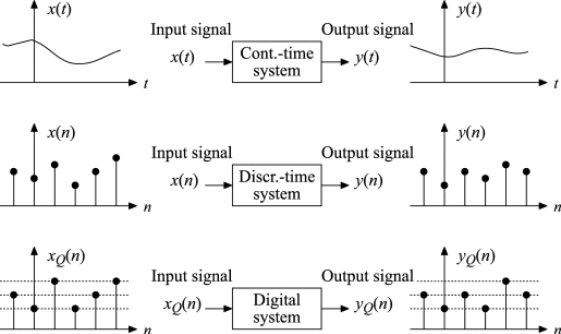
\includegraphics[width=1\linewidth]{Figura_5.png}
      \caption{\scriptsize Señal/sistema en tiempo continuo, discreto y digital (con cuantización).}
    \end{figure}
  \end{column}
\end{columns}
\end{frame}
%%%%%%%%%%%%%%%%%%%%%%%%%%%%
\begin{frame}{Frecuencia: continua vs. discreta}
\begin{columns}[T,onlytextwidth]

% --------- Continua ----------
\begin{column}{0.48\textwidth}
\begin{block}{Senoidal continua}
\small
\[
\begin{aligned}
x(t)&=A\cos(\omega t+\theta),\\
\omega&=2\pi f \quad \text{(rad/s)}
\end{aligned}
\]
\vspace{0.2em}
\begin{itemize}
  \item \textbf{Periodo}: \(T=\tfrac{1}{f}\) (siempre periódica).
  \item \textbf{Fase} \(\theta\): desplaza la onda sin cambiar \(T\).
  \item \textbf{Unidades}: \(f\) en Hz; \(\omega\) en rad/s.
\end{itemize}
\end{block}
\end{column}

% --------- Discreta ----------
\begin{column}{0.48\textwidth}
\begin{block}{Senoidal discreta}
\small
\[
\begin{aligned}
x_f[n]&=A\cos(2\pi f\,n+\theta),\\
\omega_d&=2\pi f \quad \text{(rad/muestra)}
\end{aligned}
\]
\vspace{0.2em}
\begin{itemize}
  \item \textbf{Periodicidad}: \(x[n]=x[n+N]\) \(\Leftrightarrow\) \(f\in\mathbb{Q}\).
  \item \textbf{Periodo fundamental}: si \(f=\tfrac{p}{q}\) (irreducible) \(\Rightarrow N_{\min}=q\).
  \item \textbf{Extremos}: \(f=0\) (constante), \(|f|=\tfrac12\) (máx. oscilación, \(N_{\min}=2\)).
\end{itemize}
\end{block}
\end{column}

\end{columns}
\end{frame}

%%%%%%%%%%%%%%%%%%%%%%%%%%%%
\begin{frame}{Periodicidad en discreto: resultado central}
\begin{block}{Proposición y esbozo}
  \footnotesize
\textbf{Afirmación:} \(x_f[n]\) es periódica \(\Leftrightarrow\ f\in\mathbb{Q}\).

\textit{(\(\Rightarrow\))} Si \(x_f[n]\) es \(N\)-periódica:
\[
\begin{aligned}
x_f[n]&=x_f[n+N] \\
\Rightarrow\ \cos(2\pi f n+\theta)&=\cos\!\big(2\pi f(n+N)+\theta\big) \\
\Rightarrow\ 2\pi fN&=2\pi k\ (k\in\mathbb{Z}) \\
\Rightarrow\ f&=\tfrac{k}{N}\in\mathbb{Q}.
\end{aligned}
\]

\textit{(\(\Leftarrow\))} Si \(f=\tfrac{k}{N}\) (irreducible), entonces
\[
\begin{aligned}
x_f[n+N]
&=A\cos\!\Big(2\pi\tfrac{k}{N}(n+N)+\theta\Big)
= A\cos\!\Big(2\pi\tfrac{k}{N}n+2\pi k+\theta\Big)
= x_f[n],
\end{aligned}
\]
luego \(x_f[n]\) es \(N\)-periódica.
\end{block}

\begin{alertblock}{Periodo fundamental}
Si \(f=\frac{p}{q}\) en forma irreducible, entonces \(N_{\min}=q\).  
Si \(f\notin\mathbb{Q}\), no existe \(N\) finito (aperiódica).
\end{alertblock}
\end{frame}

% =======================
\begin{frame}{Resultados en discreto: periodicidad, aliasing y definiciones}
\footnotesize
\begin{columns}[T,onlytextwidth]

% ===== Columna izquierda =====
\begin{column}{0.49\textwidth}
  \begin{block}{Proposición 1 — Periodicidad}
    Sea \(x_f[n]=A\cos(2\pi f\,n+\theta)\). Entonces
    \[
      x_f[n]\ \text{es periódica}\ \Longleftrightarrow\ f\in\mathbb{Q}.
    \]
  \end{block}

  \begin{block}{Proposición 2 — Período fundamental}
    Si \(x_f[n]\) es periódica y \(f=\tfrac{p}{q}\) en forma irreducible
    \((p,q\in\mathbb{Z},\ \gcd(p,q)=1)\), entonces
    \[
      N\big(x_f\big)=q.
    \]
  \end{block}

  \begin{block}{Definición — Período fundamental}
    Para una secuencia \(x[n]\),
    \[
      N(x)\triangleq \min\{\,N\in\mathbb{N}:\ x[n]=x[n+N]\ \forall n\,\},
    \]
    si existe; en caso contrario, \(N(x)=\infty\) (no periódica).
  \end{block}
\end{column}

% ===== Columna derecha =====
\begin{column}{0.49\textwidth}
  \begin{block}{Proposición 3 — Aliasing (redundancia)}
    Para todo \(k\in\mathbb{Z}\),
    \[
      x_{f+k}[n]=A\cos\!\big(2\pi(f+k)n+\theta\big)=A\cos(2\pi f\,n+\theta)=x_f[n].
    \]
  \end{block}

  \begin{block}{Corolario 1 — Rango de frecuencias fundamentales}
    Toda familia \(\{x_f[n]: f\in\mathbb{R}\}\) admite representantes con
    \[
      f\in\left(-\tfrac{1}{2},\,\tfrac{1}{2}\right] \qquad
      \text{(equiv. } \omega_d=2\pi f\in(-\pi,\pi]\text{)}.
    \]
    Basta restringir el análisis a ese intervalo.
  \end{block}

  \begin{block}{Definición — Frecuencia de máxima oscilación}
    En \(f\in(-\tfrac12,\tfrac12]\), la máxima oscilación ocurre en
    \[
      f^\star=\pm\tfrac{1}{2}\ \Rightarrow\ x_{f^\star}[n]=A\cos(\pi n+\theta),\quad
      N\!\left(x_{f^\star}\right)=2.
    \]
  \end{block}
\end{column}

\end{columns}
\end{frame}

%%%%%%%%%%%%%%%%%%%%%%%%
\section{Pregunta 1}
\begin{frame}{Pregunta \#1}
\begin{block}{Enunciado Pregunta \#1}
  \footnotesize
   Responda lo siguiente:
\begin{enumerate}

  \item Demuestre que una señal coseno discreta es periódica si y sólo si la frecuencia es racional:
  \begin{equation}
    (x(n))_{n\in\mathbb{Z}}
    =\bigl(A\cos(2\pi f\,n+\varphi)\bigr)_{n\in\mathbb{Z}}
    \quad\Longleftrightarrow\quad f\in\mathbb{Q}.
  \end{equation}

  \item Considere la siguiente familia de señales exponenciales:
  \begin{equation}
    (s_k(n))_{n\in\mathbb{Z}}
    =\left(e^{\,\mathrm{j}\frac{2\pi k}{N}\,n}\right)_{n\in\mathbb{Z}},
    \qquad k=0,1,2,\ldots
  \end{equation}
  Muestre que su período fundamental está dado por
  \begin{equation}
    N_p \;=\; \frac{N}{\gcd(k,N)},
  \end{equation}
  donde \(\gcd(\cdot,\cdot)\) denota el máximo común divisor.
\end{enumerate}
\end{block}
\end{frame}
%%%%%%%%%%%%%%%%%%%%%%
\section{Pregunta 2}
\begin{frame}{Pregunta \#2}
\begin{block}{Enunciado Pregunta \#2}
Determine si las siguientes señales son periódicas. Si corresponde, especifique su período fundamental.
\begin{enumerate}
  \item \(x_a(t)=6\cos\big(9t+\tfrac{\pi}{3}\big)\).
  \item \(x(n)=6\cos\big(9n+\tfrac{\pi}{3}\big)\).
  \item \(x(n)=\cos\!\big(\tfrac{n}{8}\big)\,\cos\!\big(\tfrac{\pi n}{8}\big)\).
  \item \(x(n)=2\,e^{\,j\left(\tfrac{\pi}{7}n-3\right)}\).
  \item \(x(n)=\cos\!\big(\tfrac{\pi n}{2}\big)-\sin\!\big(\tfrac{\pi n}{8}\big)+3\cos\!\big(\tfrac{\pi n}{4}+\tfrac{\pi}{3}\big)\).
\end{enumerate}
\end{block}
\end{frame}
%%%%%%%%%%%%%%%%%%%%%%
\begin{frame}
\begin{figure}
  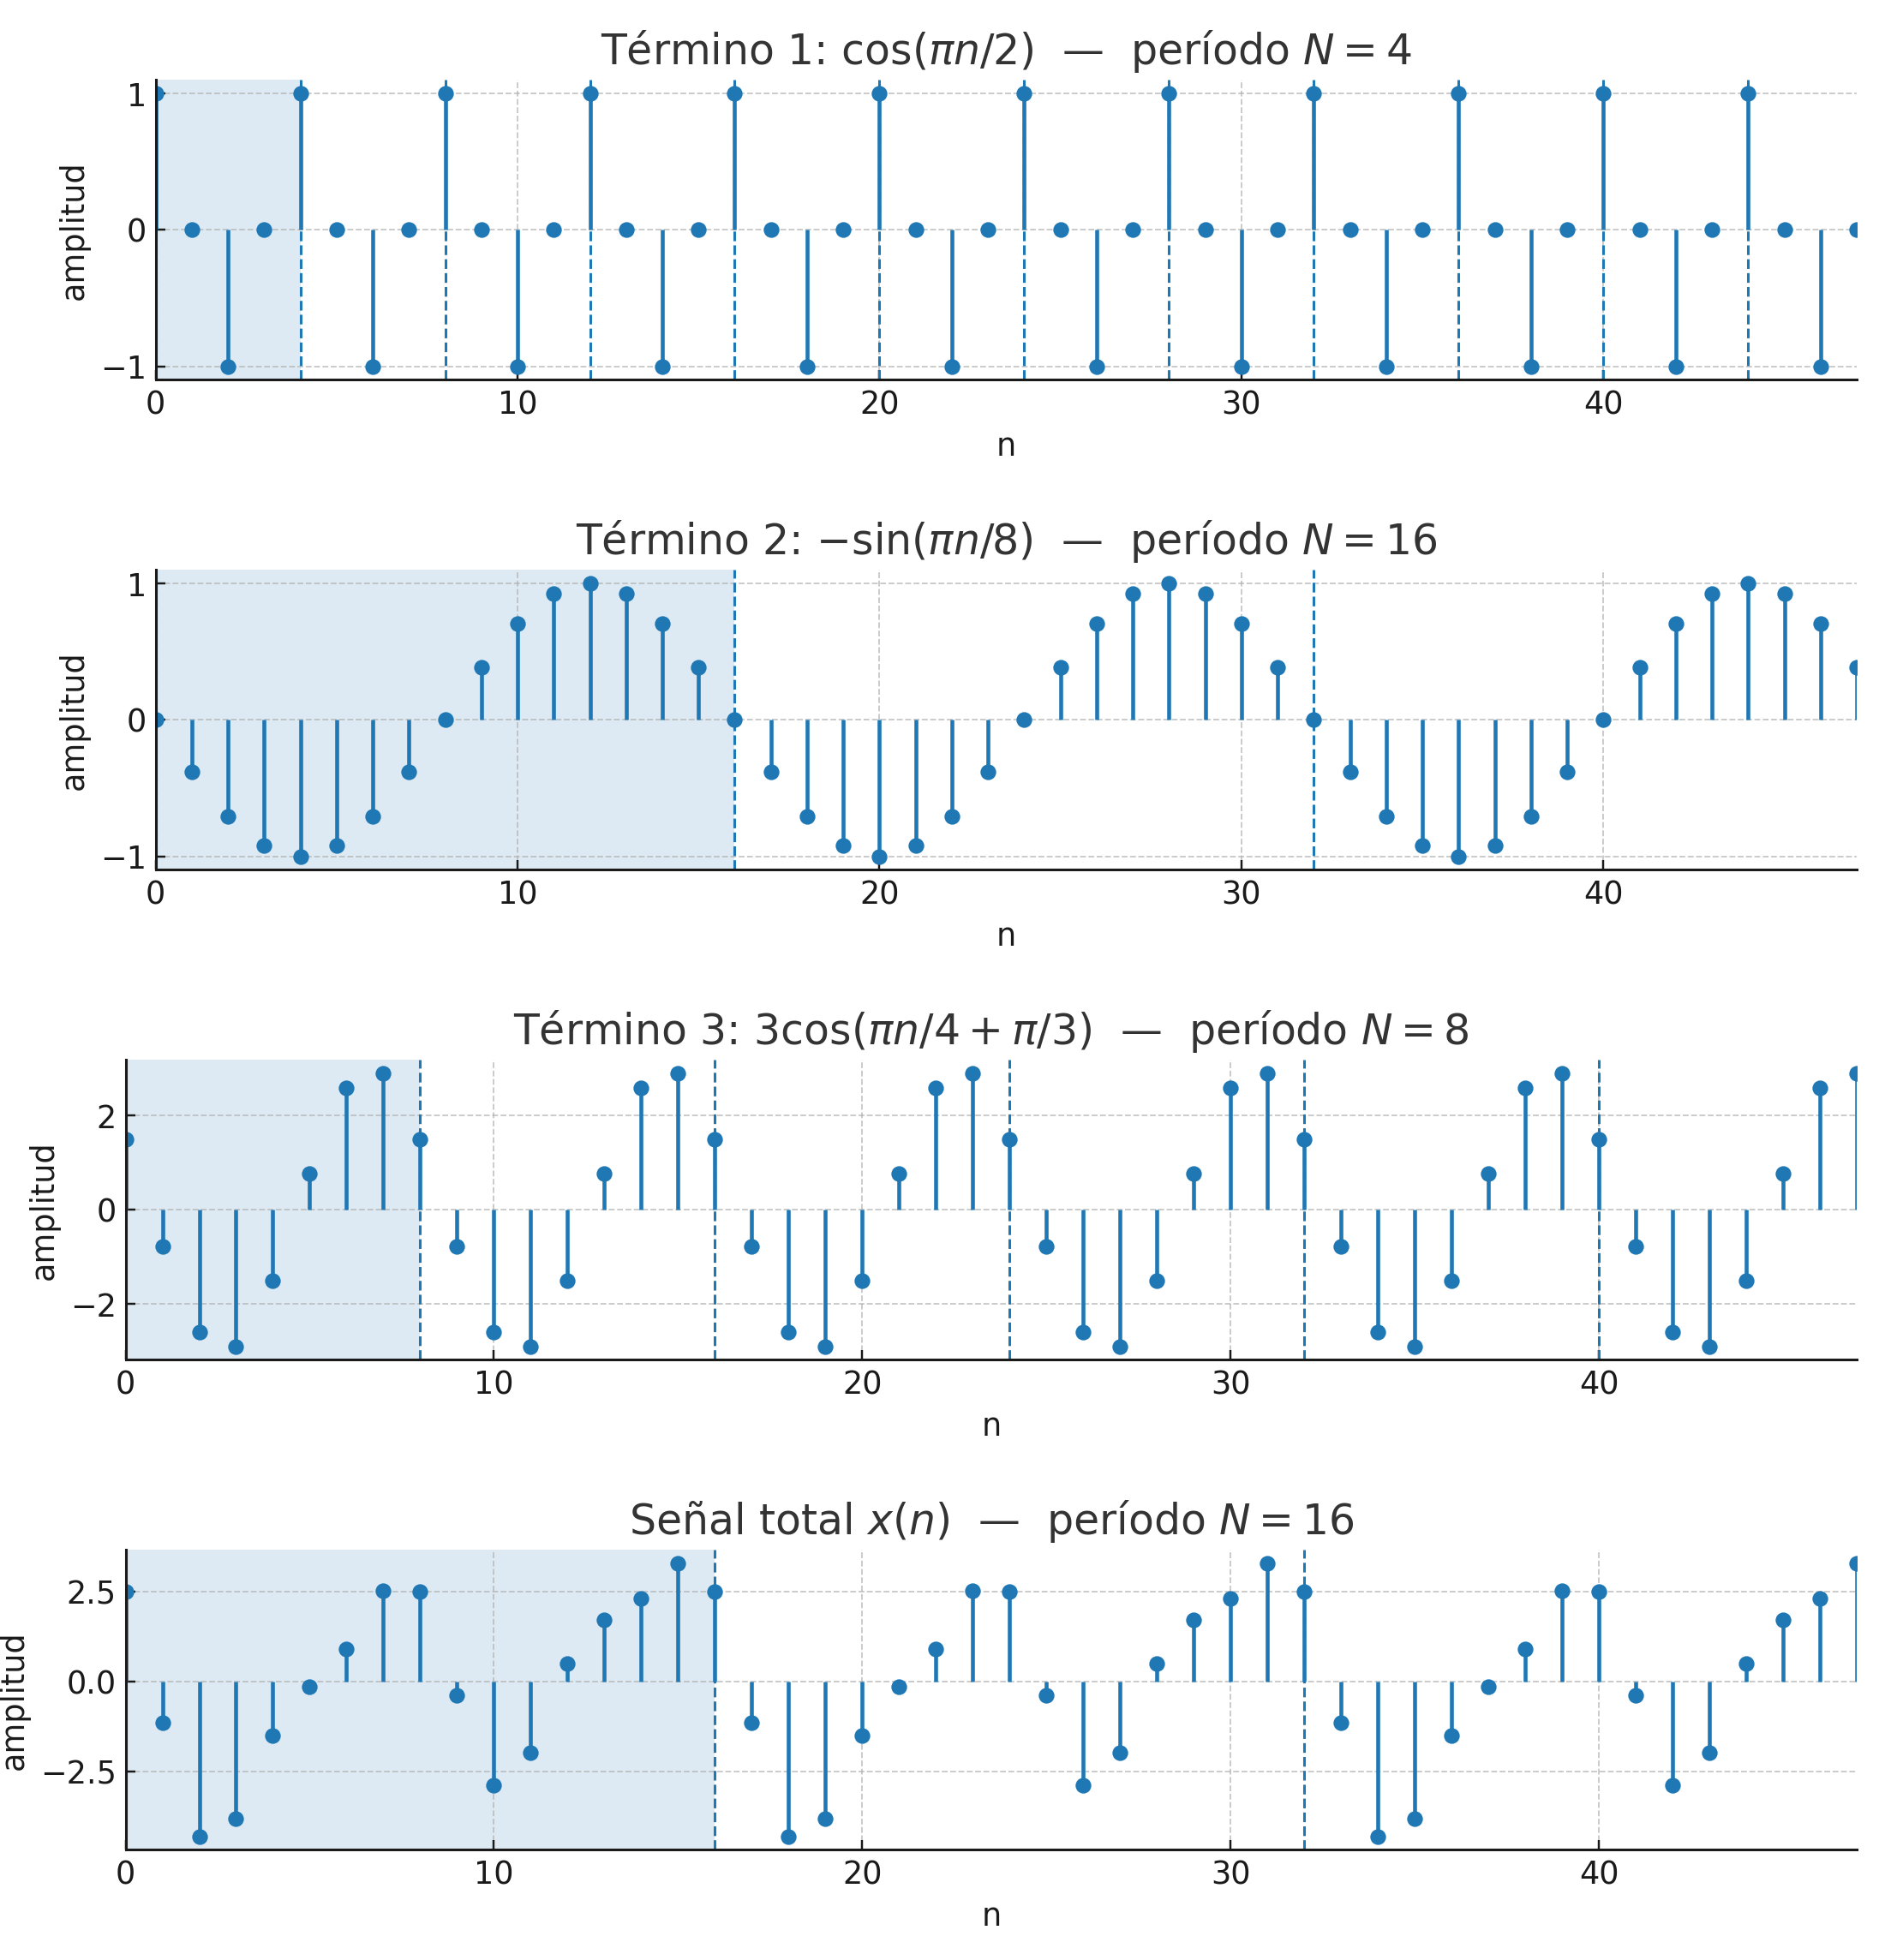
\includegraphics[width=0.52\textwidth]{Auxiliar_1_1.png}
\end{figure}
\end{frame}
%%%%%%%%%%%%%%%%%%%%%%
\section{Pregunta 3}
\begin{frame}{Pregunta \#3}
\begin{block}{Enunciado Pregunta \#3}
Considere la siguiente señal sinusoidal a tiempo continuo:
\begin{equation}
  x_a(t) \;=\; \frac{7}{2}\,\sin(200\pi\,t), 
  \qquad t \in \mathbb{R}.
\end{equation}

\begin{enumerate}
  \item Bosqueje \(x_a(t)\) para \(0 \le t \le 30\,\text{ms}\).
  \item La señal \(x_a(t)\) es muestreada a una tasa de \(F_s=300\,\text{Hz}\).
        Determine la frecuencia de la señal a tiempo discreto \(x[n]=x_a(nT_s)\),
        donde \(T_s = 1/F_s\). 
        Muestre que \(x[n]\) es periódica y determine su período fundamental.
  \item Bosqueje la señal \(x[n]\) en el mismo diagrama donde bosquejó \(x_a(t)\).
        ¿Cuál es el equivalente en milisegundos del período de \(x[n]\)?
\end{enumerate}
\end{block}
\end{frame}
%%%%%%%%%%%%%%%
\begin{frame}
  \begin{block}{Bosquejo de señal continua}
  \end{block}
  \begin{figure}
    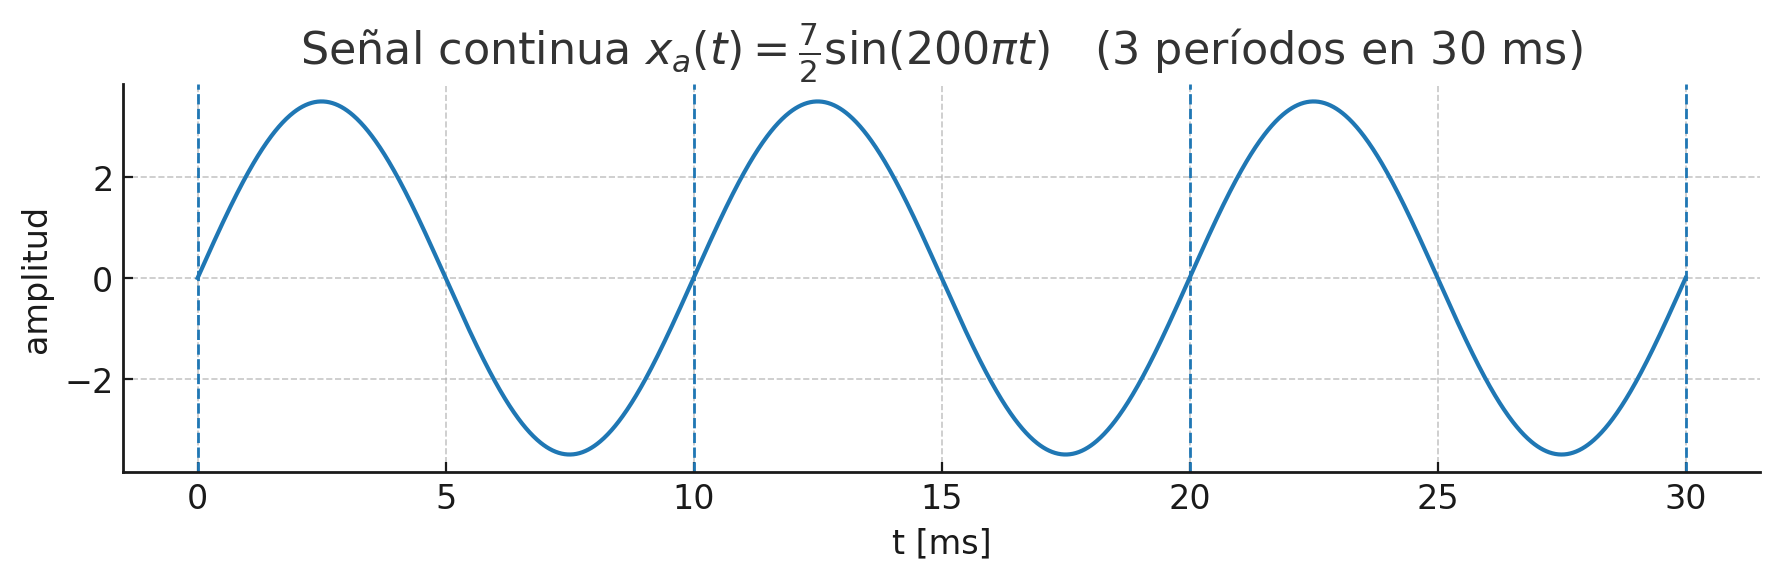
\includegraphics[width=0.8\textwidth]{Auxiliar_1_2.png}
  \end{figure}
\end{frame}
%%%%%%%%%%%%%%%%%%%%%%
\begin{frame}
  \begin{block}{Bosquejo de señal discreta}
     \end{block}
    \begin{figure}
    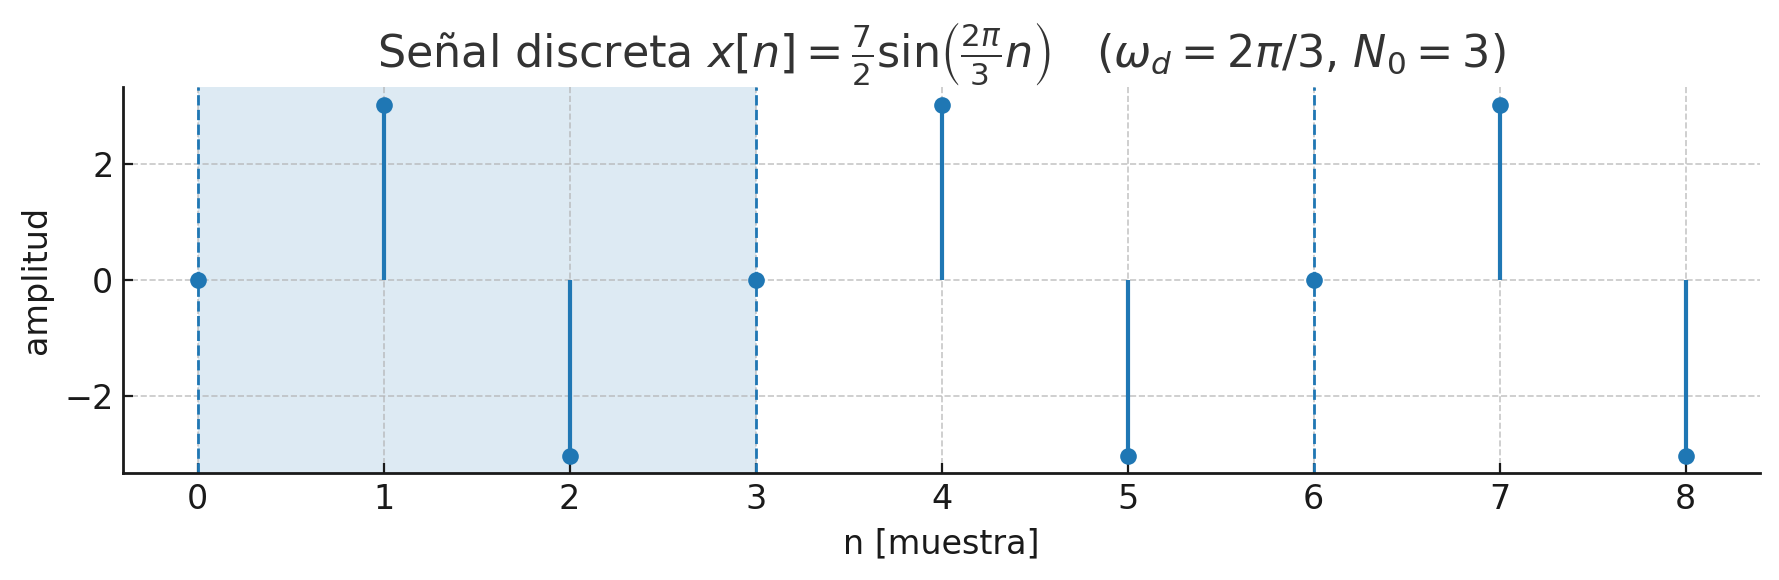
\includegraphics[width=0.8\textwidth]{Auxiliar_1_3.png}
  \end{figure}
\end{frame}
%%%%%%%%%%%%%%%%%%%%%%
\begin{frame}
  \begin{block}{Bosquejo de señal discretizada}
  \end{block}
  \begin{figure}
    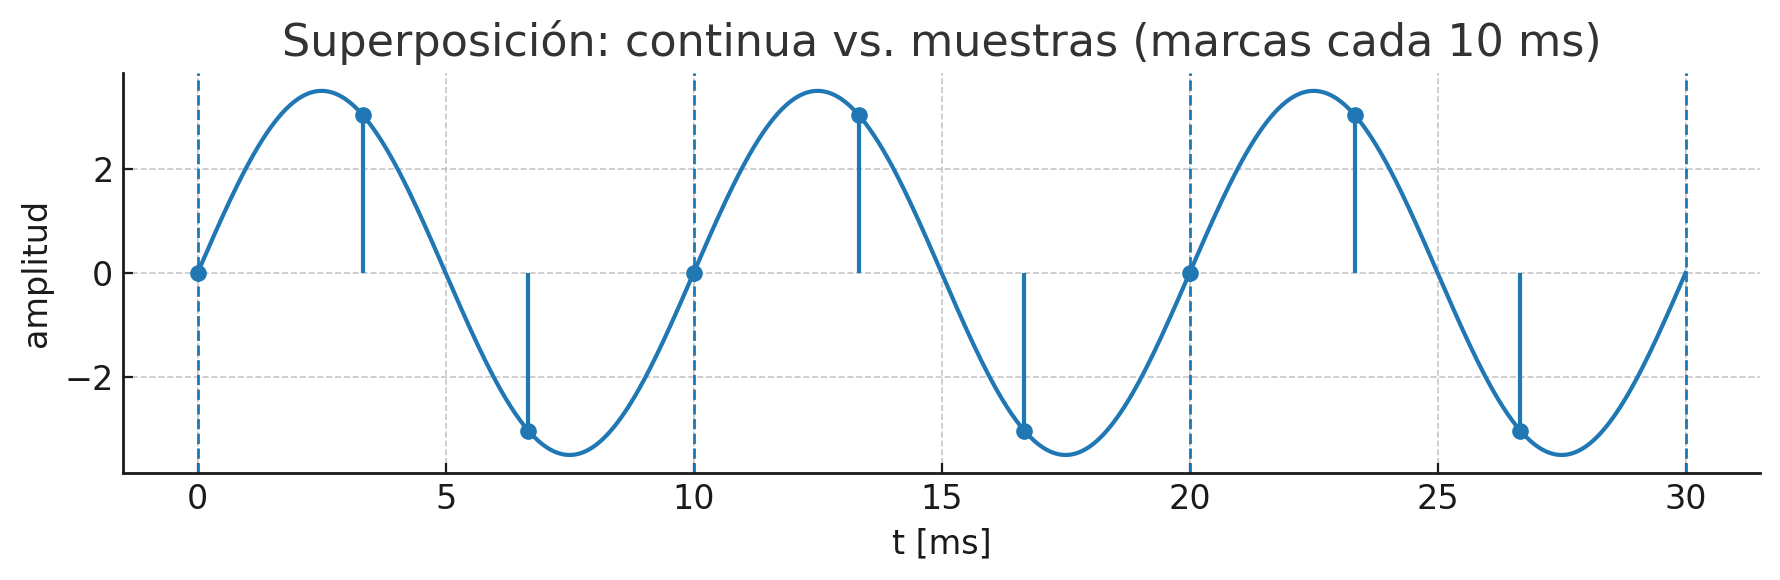
\includegraphics[width=0.8\textwidth]{Auxiliar_1_4.png}
  \end{figure}
\end{frame}
%%%%%%%%%%%%%%%%%%%%%%
\section{Pregunta 4}
\begin{frame}{Pregunta \#4}
\begin{block}{Enunciado Pregunta \#4}
Considere una señal continua \(x_a(t)\) periódica con período fundamental \(T_a\) (en segundos).

\begin{enumerate}
  \item Si se muestrea la señal \(x_a(t)\) a una tasa constante de \(F_s\) muestras por segundo, es decir, se induce la señal discreta
  \begin{equation}
    x[n] \;=\; x_a\!\left(\frac{n}{F_s}\right), \qquad \forall\, n\in\mathbb{Z},
  \end{equation}
  encuentre la(s) condición(es) que garantice(n) que \(x[n]\) sea periódica y, con ello, determine su período fundamental.

  \item Con base en el punto anterior, justifique la siguiente afirmación:
  si \(x[n]\) es periódica, entonces su período fundamental (equivalente en \textbf{segundos}) es un múltiplo de \(T_a\).
\end{enumerate}
\end{block}
\end{frame}

\end{document}
